The first step is to compare the performance of Apache and Nginx web serving software. However, it is not necessary to compare these software in their speed of serving static content (for example HTML files) because it has been proven and because of Nginx architecture that Nginx is more performant in this manner.

What is interesting to compare, though, is running of PHP under Apache and Nginx.

\section{Apache with mod\_php}

"Apache supports a variety of features, many implemented as compiled modules which extend the core functionality." "Instead of implementing a single architecture, Apache provides a variety of MultiProcessing Modules (MPMs), which allow Apache to run in a process-based, hybrid (process and thread) or event-hybrid mode, to better match the demands of each particular infrastructure." \cite{Apache:Wiki}\\

In a default configuration, when HTTP requests are received, Apache starts to process them one by one. It spawns multiple child processes to handle the load. However, these proccesses are standalone, meaning they initialize all modules (including mod\_php) even for static file requests. This behavior results in high RAM usage as seen on figure \ref{fig:apache_mod_php}. \\

mod\_php is a PHP interpreter module for Apache. It is the most common way of executing PHP scripts when using Apache HTTP. The module is loaded in each Apache process, thus a request for a PHP script is executed directly within the process, not being relayed to another server with the ability to run the script. The main disadvantage to embedding PHP inside Apache is that if a user is requesting a static resource such as CSS, JS or an image, it still has to go through Apache process with PHP module, therefore increasing RAM and CPU usage.

\subsection{Load testing Apache with mod\_php}

We are going to load test Apache with mod\_php running a simple WordPress-powered site. Within your command line, navigate to the wordpress-ansible directory and run the "apache\_mod\_php.yml" Ansible playbook:


\begin{lstlisting}
ansible-playbook -i hosts apache_mod_php.yml
\end{lstlisting}

The playbook will configure Apache and create a virtual host for the WordPress site. We are using a default Apache HTTP configuration file without any performance modifications. \cite{WP_Ansible:apache.conf}\\

To deploy the simple WordPress site, run the "wordpress\_basic.yml" Ansible playbook. It will download the latest version of WordPress with the default theme and installs the database tables. We are now ready to carry out the testing. \\

At the loader.io load testing service, we have created a new test \cite{Loader.io:apache_mod_php}, configuring it to send from 0 to 200 simultaneous client requests to the index of our testing server for a duration of 30 seconds. Figure \ref{fig:apache_mod_php} depicts the final chart.


\begin{figure}[H]
\begin{center}
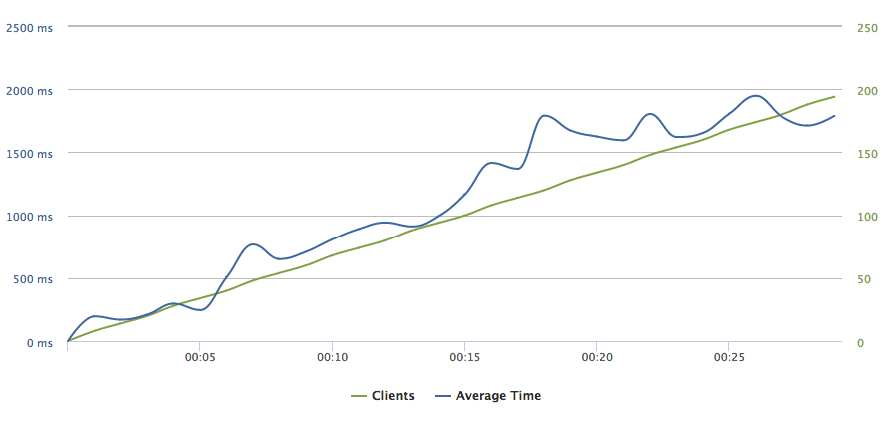
\includegraphics[scale=0.5]{figures/Apache_mod_php.png}
\caption{Apache HTTP with mod\_php: clients versus average response time}
\label{fig:apache_mod_php}
\end{center}
\end{figure}

This chart shows the average server response times when a number of simultaneous client requests are sent to it. We can observe that even under a high load of 200 concurrent requests the average response time is under 2 seconds. It grows approximately linearly. \\

However, to truly see how the server copes with the load, the figures \ref{fig:apache_mod_php_2s} and \ref{fig:apache_mod_php_25s} come in handy. They represent screenshots of Htop interactive process viewer \cite{Htop:main_site} during 2 and 25 seconds into the load testing, respectively.

\begin{figure}[H]
\begin{center}
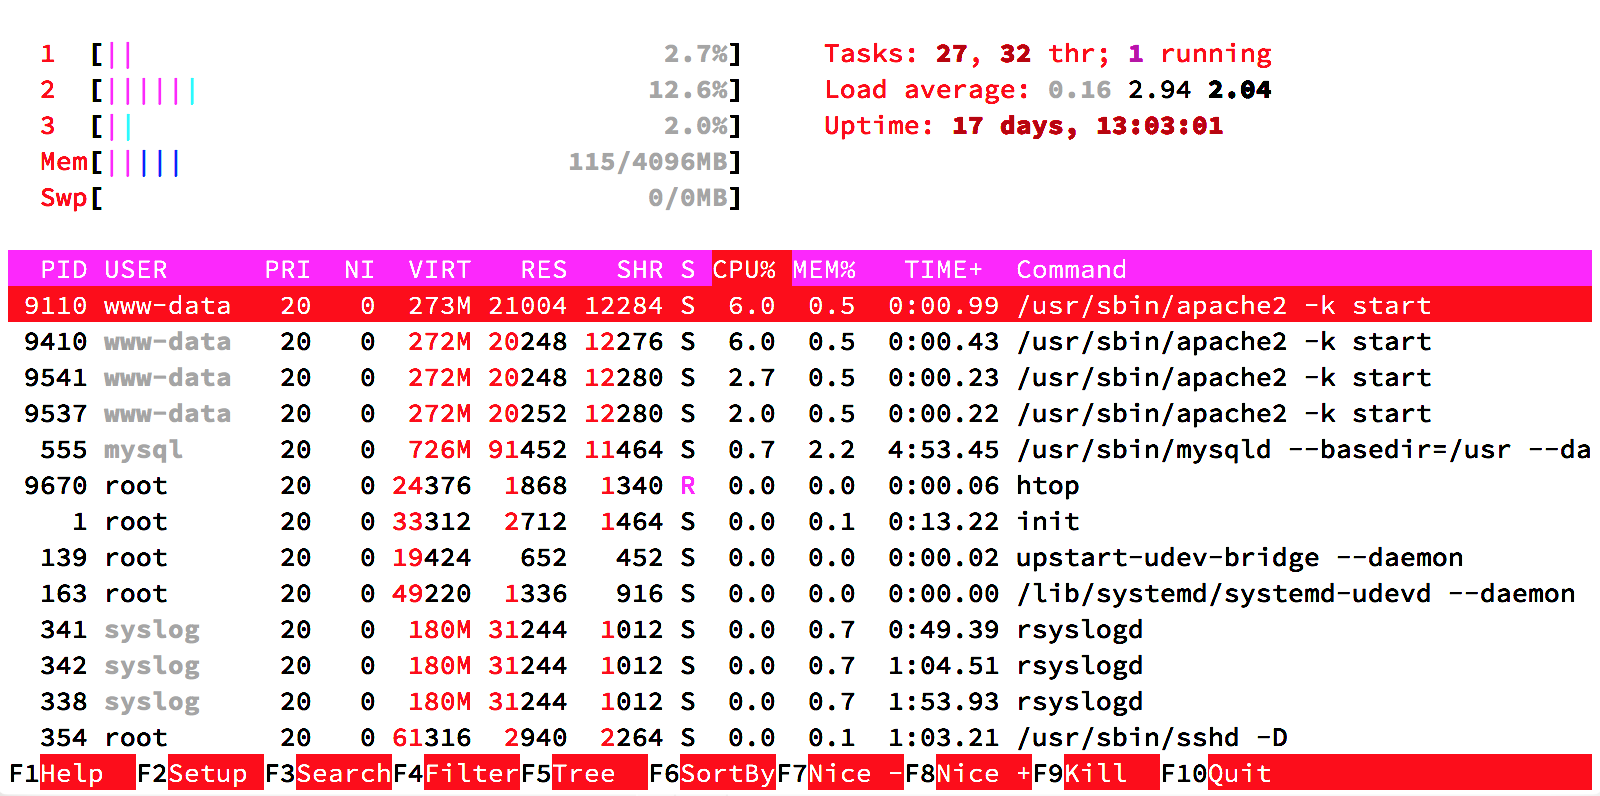
\includegraphics[scale=0.5]{figures/Apache_mod_php_2s.png}
\caption{Apache HTTP with mod\_php: Htop process viewer 2 seconds into test}
\label{fig:apache_mod_php_2s}
\end{center}
\end{figure}

On the screenshot, we can see a table of currently running processes. The columns RES, CPU\% and MEM\% show the RAM usage in kilobytes, CPU usage in percentage and RAM usage in percentage of a process, respectively. What is more, there are several gauges, visually depicting the usage or particular CPU core (or thread), RAM and Linux Swap. Opening the Htop's help screen (F1 in Htop), the gauges are explained as follows:

\begin{figure}[H]
\begin{center}
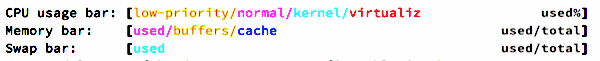
\includegraphics{figures/htop_help_gauges.png}
\caption{Screenshot of Htop's help screen explaining the main gauges}
\label{fig:htop_help_gauges}
\end{center}
\end{figure}

It is crucial to notice that the yellow bars in the Memory bar section show cached memory, which is not counted towards the used memory since it can be misleading at times (will discuss this a bit later).

\begin{figure}[H]
\begin{center}
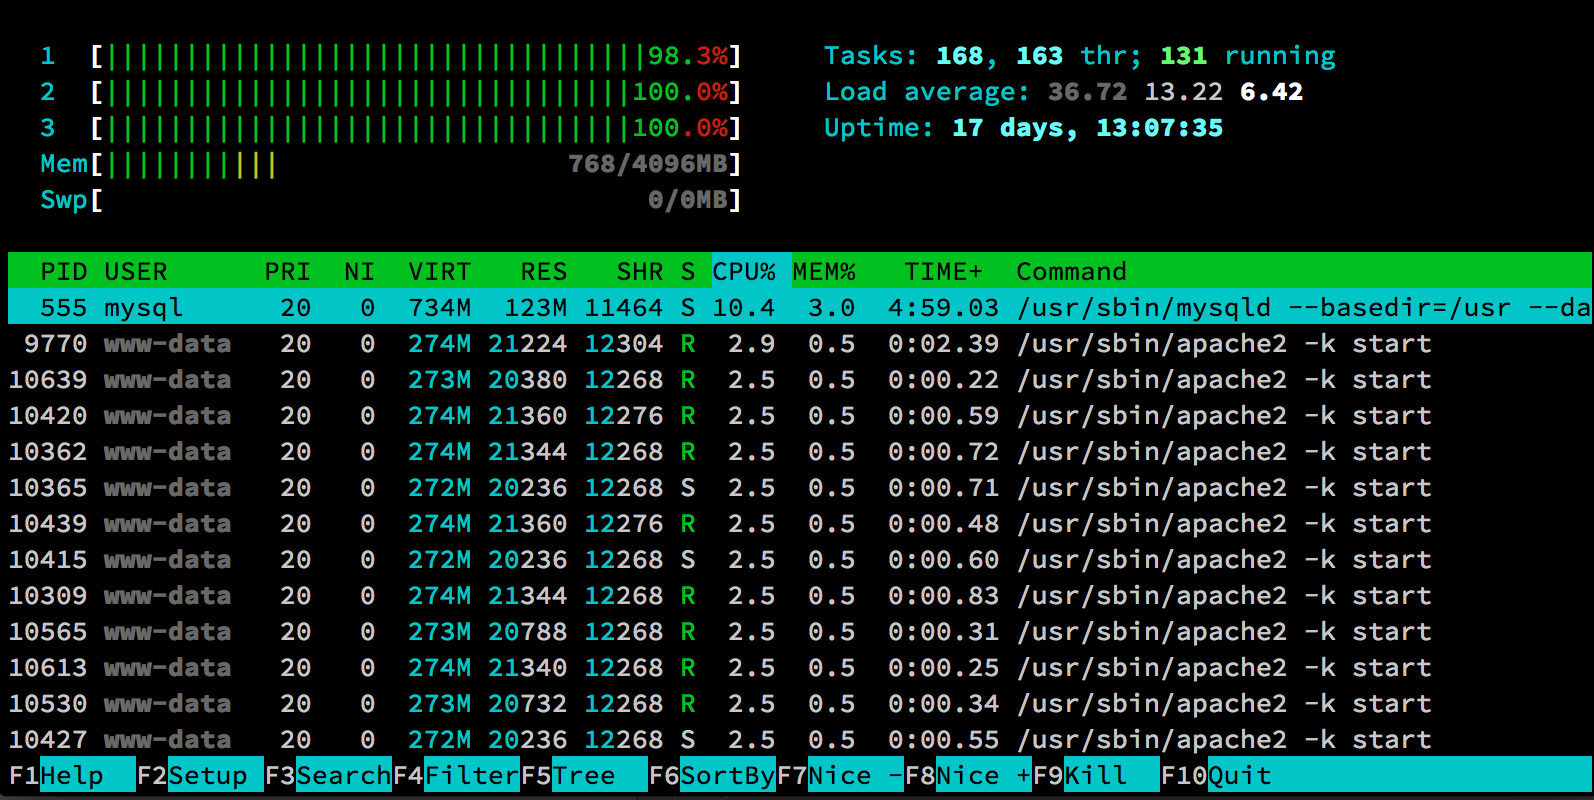
\includegraphics[scale=0.5]{figures/Apache_mod_php_25s.png}
\caption{Apache HTTP with mod\_php: Htop process viewer 25 seconds into test}
\label{fig:apache_mod_php_25s}
\end{center}
\end{figure}

From both screenshots, we can observe that Apache HTTP, represented by the process /usr/sbin/apache2 is, at first, just warming up, spawning three child processes and under heavy load, consuming the CPU completely and taking about 770 megabytes of memory. It does not tell us much without comparing it to the results of benchmarking different server stacks, what we are going to do shortly. \\

Loader.io testing results page \cite{Loader.io:apache_mod_php} also shows us more statistics about the test:

\begin{itemize}
	\item\textbf{Average response time:} 1229 ms
	\item\textbf{Min/Max response times:} 144 / 4660 ms
	\item\textbf{Count of successful responses:} 2178
\end{itemize}

\section{Nginx with PHP-FPM}

"Nginx (pronounced "engine-x") is an open source [...] web server. The nginx project started with a strong focus on high concurrency, high performance and low memory usage. [...] Nginx uses an asynchronous event-driven approach to handling requests, instead of the Apache HTTP Server model that defaults to a threaded or process-oriented approach, where the Event MPM is required for asynchronous processing. Nginx's modular event-driven architecture can provide more predictable performance under high loads." \cite{Nginx:Wiki} \\

Due to Nginx's asynchronous event-driven nature, its primary use case scenario is to relay the incoming requests to another application for processing, such as PHP-FPM, as quickly as possible, thus being able to handle large amounts of concurrent connections. \\

PHP-FPM is a FastCGI server bound to a TCP port or socket, bundled with the official PHP interpreter. It listens for PHP requests (request for a PHP script), responding with the resulting content (usually HTML). Comparing Apache's mod\_php with PHP-FPM, while a PHP request is processed by Apache directly, in case of Nginx, it has to be relayed to PHP-FPM, which is able to process it. We do not have to know how it works in a greater depth to understand that when a request is flowing through multiple applications, more server resources have to be consumed. On the other hand, as Nginx and PHP-FPM are specialized applications, they are more efficient when put together. It can be observed on the figures below.

\subsection{Load testing Nginx with PHP-FPM}

Within your command line, navigate to the wordpress-ansible directory and run the "nginx\_php-fpm.yml" Ansible playbook:

\begin{lstlisting}
ansible-playbook -i hosts nginx_php-fpm.yml
\end{lstlisting}

Analogous to the load testing Apache with mod\_php, we create a new test on Loader.io with the same configuration. \cite{Loader.io:nginx_php-fpm}

\begin{figure}[H]
\begin{center}
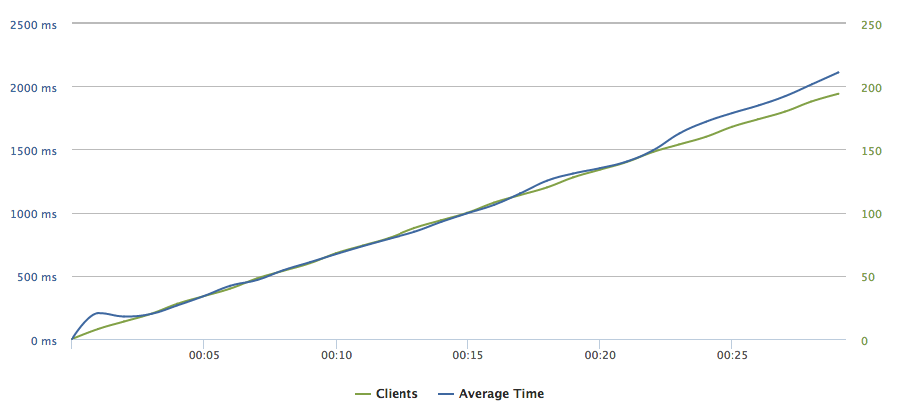
\includegraphics[scale=0.5]{figures/Nginx_PHP-FPM.png}
\caption{Nginx with PHP-FPM: clients versus average response time}
\label{fig:nginx_php-fpm}
\end{center}
\end{figure}

Figure \ref{fig:nginx_php-fpm} shows us similar average response times to the figure \ref{fig:apache_mod_php} (Apache with mod\_php), even slightly worse. However, screenshots of Htop during 1 and 22 seconds into the test depict a different situation. As we can see, even under 150 simultaneous client requests, server RAM usage is only at 46 MB. Compared with Apache's 770 MB, by installing Nginx with PHP-FPM we optimized the server markedly. We can also see that Nginx is not using more than 3\% of the server's CPU for the reason that it was programmed to manage thousands of concurrent connections and we sent only 200 of them. Better benchmark for Nginx performance is described in the \ref{page-caching} section. \\

Although we could tweak Apache with mod\_php to have a better performance, it has a steep learning curve, requiring a considerable amount of time. The objective of this work is to provide web administrators and WordPress developers with solutions they can easily implement, therefore we will not elaborate on this topic in greater detail. 

\begin{figure}[H]
\begin{center}
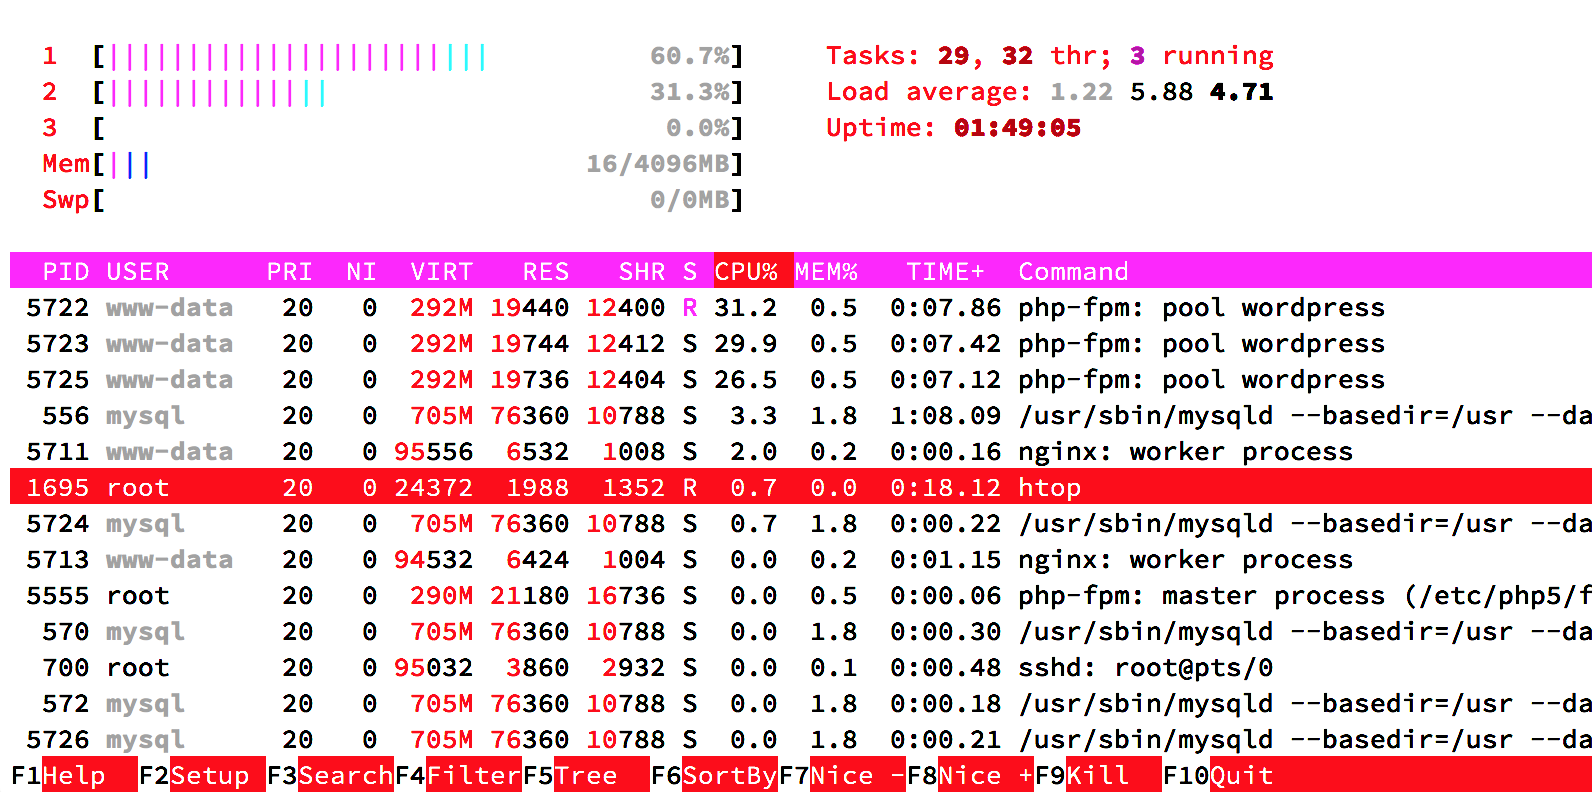
\includegraphics[scale=0.5]{figures/Nginx_PHP-FPM_1s.png}
\caption{Nginx with PHP-FPM: Htop process viewer 1 second into test}
\label{fig:nginx_php-fpm_1s}
\end{center}
\end{figure}

\begin{figure}[H]
\begin{center}
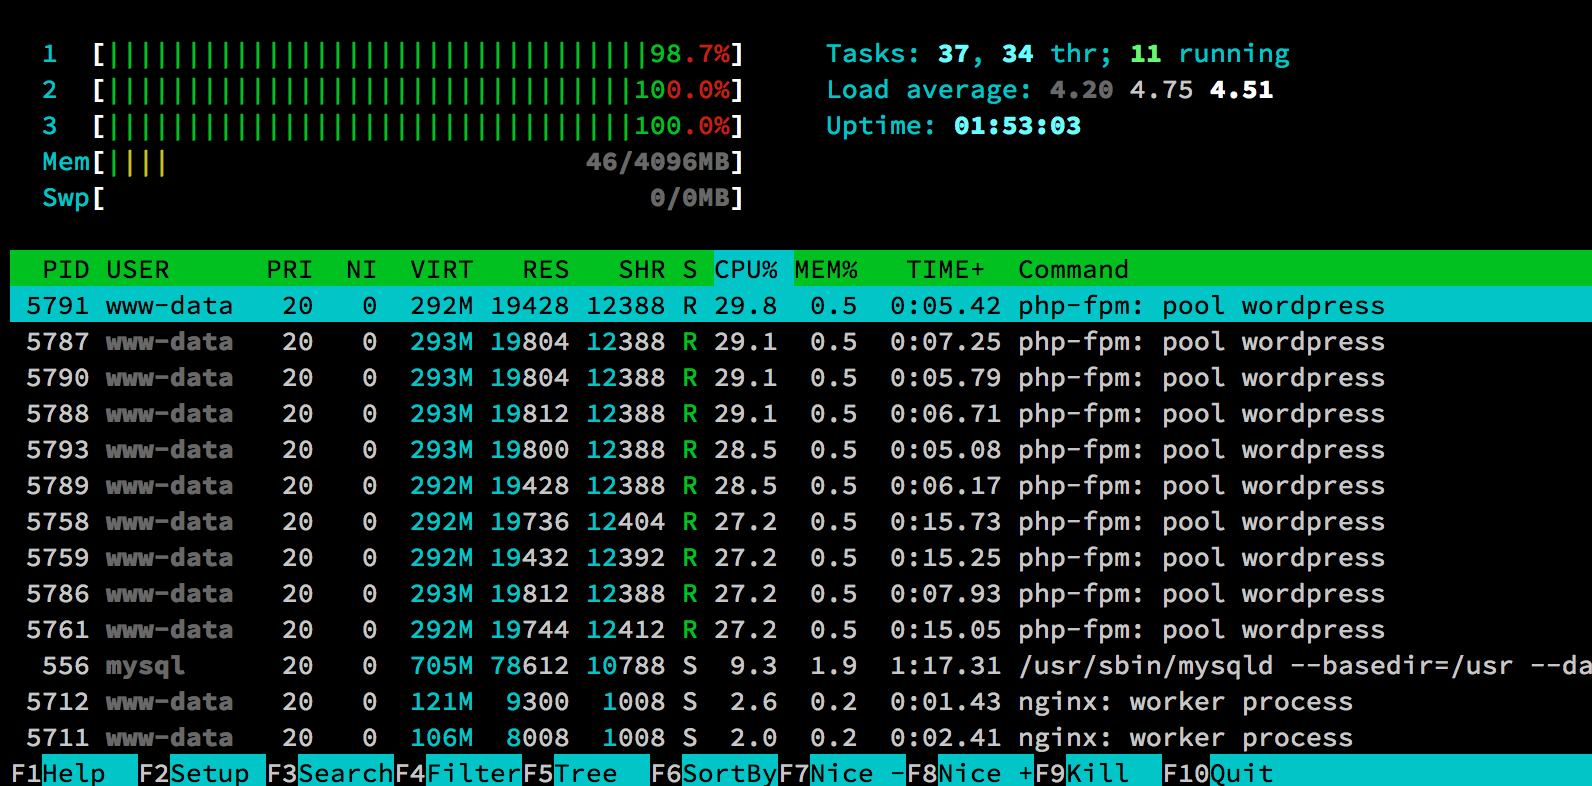
\includegraphics[scale=0.5]{figures/Nginx_PHP-FPM_22s.png}
\caption{Nginx with PHP-FPM: Htop process viewer 22 seconds into test}
\label{fig:nginx_php-fpm_22s}
\end{center}
\end{figure}

Astute readers might notice that MariaDB process (/usr/sbin/mysqld) consumes more memory (RES column) than Htop's Mem gauge total used memory is showing (46 MB) alone. As we have explained from the figure \ref{fig:htop_help_gauges}, memory bar is not counting the cached memory to its total used value. The only indication is the yellow bars which follow the green ones.

\section{Nginx + HHVM}

In this section, we are going to substitute PHP-FPM with a different FastCGI PHP interpreter, HHVM and load-test it as we did with the earlier technologies. \\

"HipHop Virtual Machine (HHVM) is a process virtual machine based on just-in-time (JIT) compilation, serving as an execution engine for PHP. [...] By using the principle of JIT compilation, executed PHP [...] code is first transformed into intermediate HipHop bytecode (HHBC), which is then dynamically translated into the x86-64 machine code, optimized and natively executed. This contrasts to the PHP's usual interpreted execution, in which the Zend Engine transforms the PHP source code into opcodes as a form of intermediate code, and executes the opcodes directly on the Zend Engine's virtual CPU.". \cite{HHVM:Wiki} \\

\subsection{Load testing Nginx with HHVM}

Within your command line, navigate to the wordpress-ansible directory and run the "nginx\_hhvm.yml" Ansible playbook:

\begin{lstlisting}
ansible-playbook -i hosts nginx_hhvm.yml
\end{lstlisting}

Analogous to the load testing Apache with mod\_php, we create a new test on Loader.io with the same configuration. \cite{Loader.io:nginx_hhvm} As HHVM is transforming and optimizing the PHP code during the initial requests, we have made several ones before running the load testing to get more accurate results (response time for the initial request was more than 10 seconds long).

\begin{figure}[H]
\begin{center}
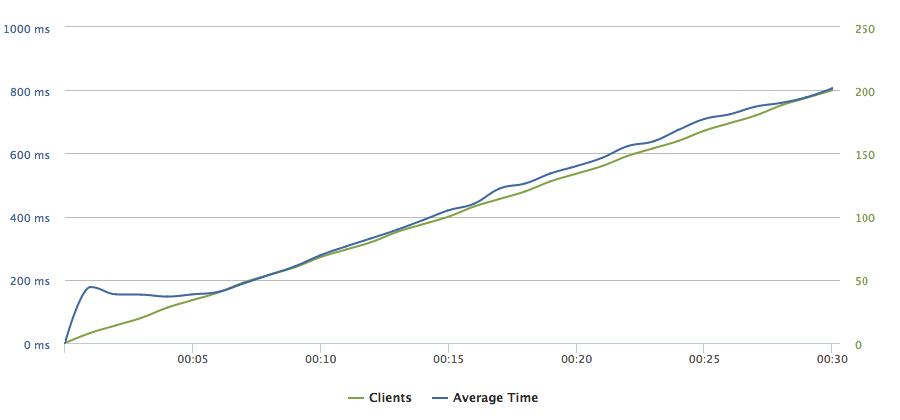
\includegraphics[scale=0.5]{figures/Nginx_HHVM.png}
\caption{Nginx with HHVM: clients versus average response time}
\label{fig:nginx_hhvm}
\end{center}
\end{figure}

Reviewing the above chart, we can see that average response times have decreased from the 2-second to under 1-second levels. When 200 simultaneous requests are sent to the server, we receive them after 800 ms in average. This means that just by using HHVM instead of PHP-FPM, the performance of our server increases 2,5 times. What is more, the count of successful responses leaps to around 5800, thus nearly tripling the throughput of the server. \cite{Loader.io:nginx_hhvm}

\begin{figure}[H]
\begin{center}
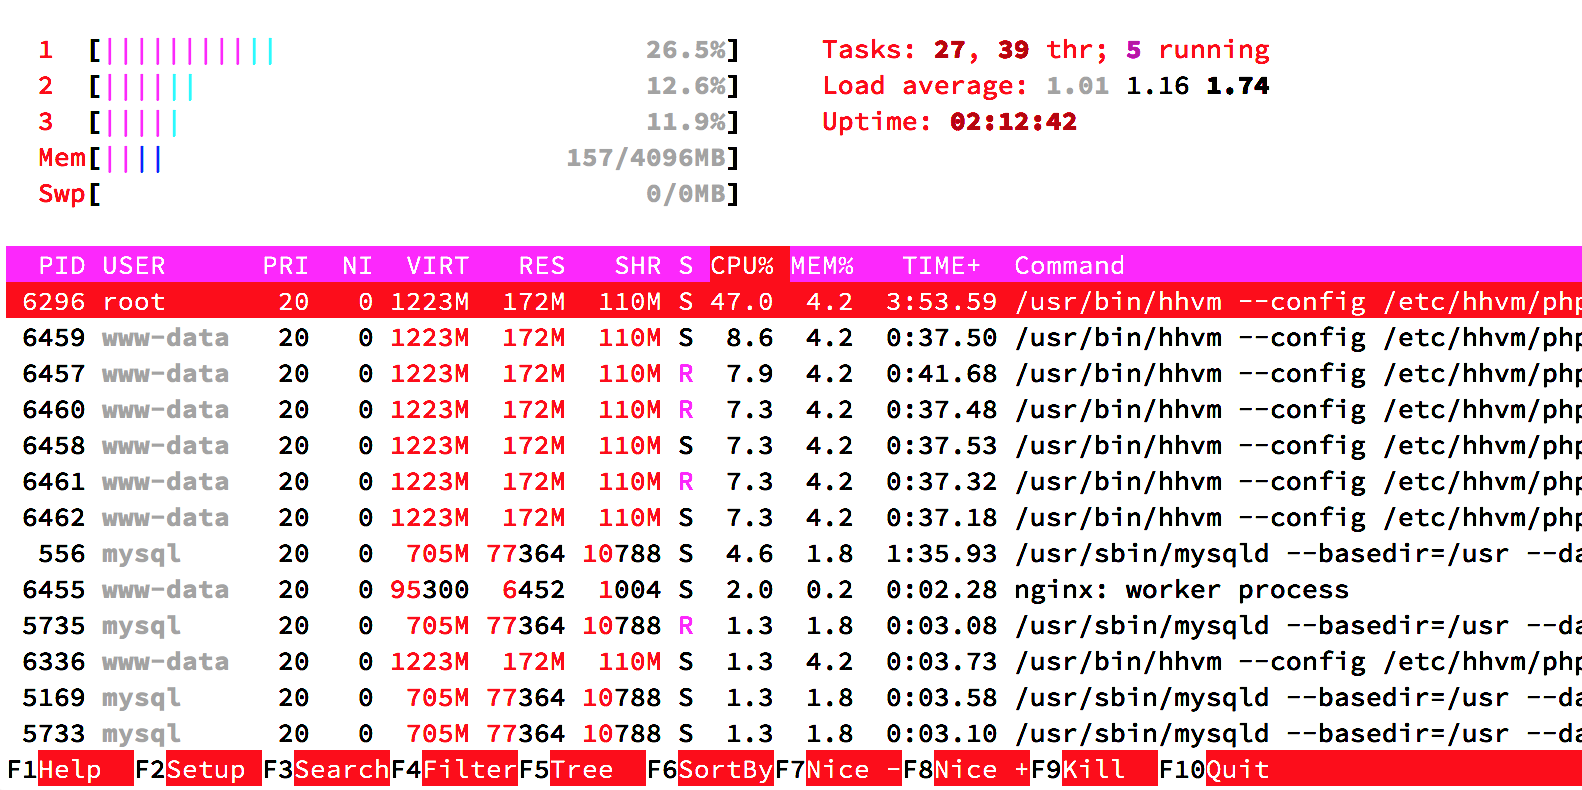
\includegraphics[scale=0.5]{figures/Nginx_HHVM_1s.png}
\caption{Nginx with HHVM: Htop process viewer 1 second into test}
\label{fig:nginx_hhvm_1s}
\end{center}
\end{figure}

\begin{figure}[H]
\begin{center}
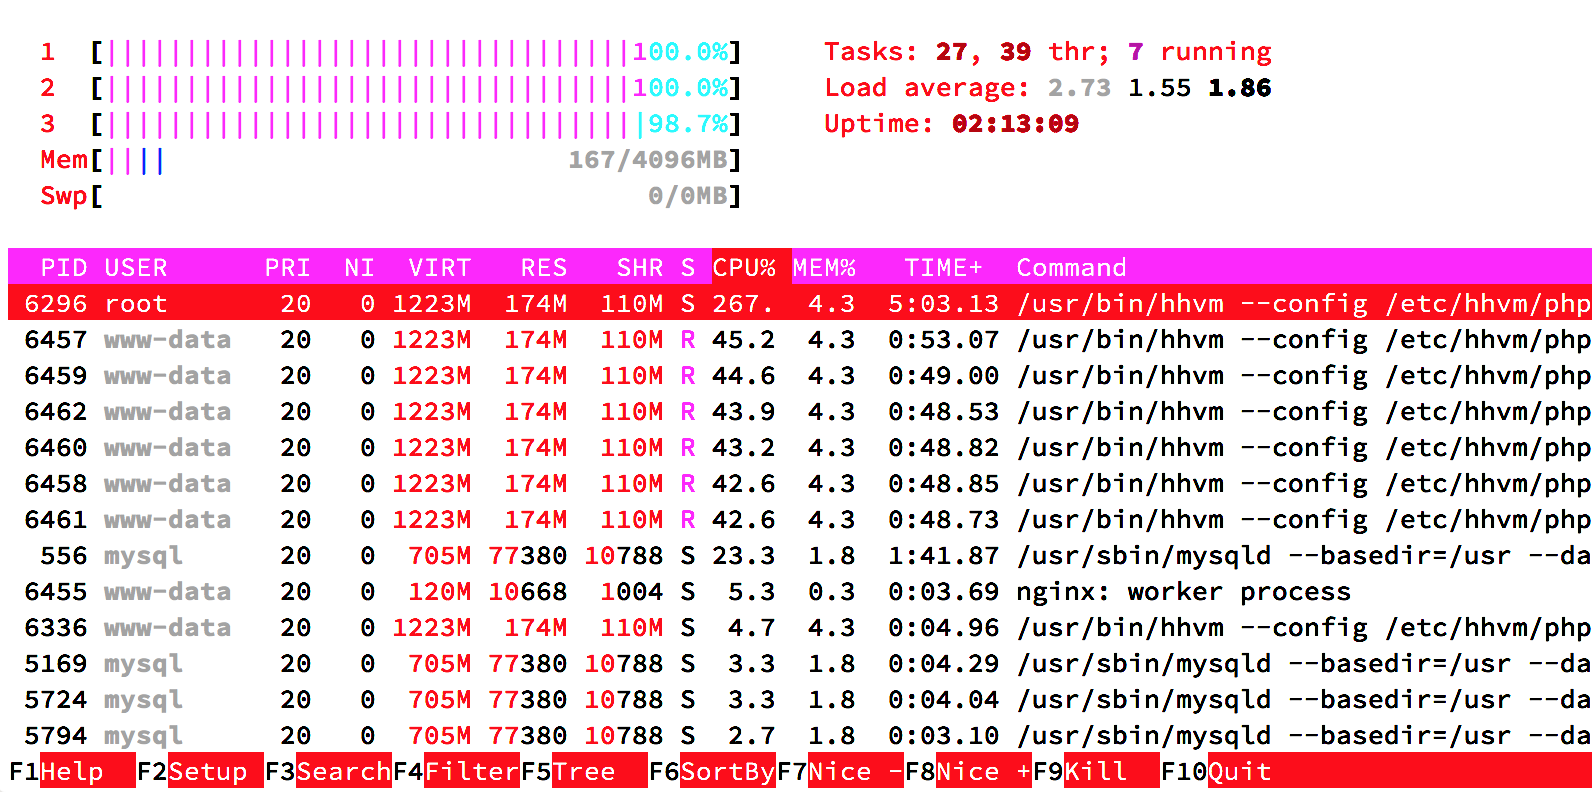
\includegraphics[scale=0.5]{figures/Nginx_HHVM_24s.png}
\caption{Nginx with HHVM: Htop process viewer 22 seconds into test}
\label{fig:nginx_hhvm_24s}
\end{center}
\end{figure}

Looking at the Htop process viewer screenshot, in comparison to using PHP-FPM, RAM usage more than tripled. However, it is still relatively low, especially compared to the memory usage when using Apache with mod\_php. \\

If this was a competition, choosing Nginx with HHVM as your web-serving stack would beat all its contestants, therefore we recommend going with it.

